\chapter{\texorpdfstring{\ds/\dpl production-yield ratio}{Ds+/D+ production-yield ratio}}\label{ch:results}
The \pt-differential \ds/\dpl production-yield ratio can be evaluated using the quantities obtained in Chapters~\ref{chap:RY} and~\ref{ch:corrections}. The \ds/\dpl production-yield ratio is defined using Eq.~\ref{eq:DsDplusRatio}, here reported for convenience:
\begin{equation*}
    \ds/\dpl = \frac{N_\mathrm{raw}^{\ds}\cdot \fpds}{\aeffpds \cdot \mathrm{BR}^\ds} \cdot \left(\frac{N_\mathrm{raw}^{\dpl}\cdot \fpdpl}{\aeffpdpl \cdot \mathrm{BR}^\dpl}\right)^{-1}\quad .
\end{equation*}
Previous measurements have been performed at different centre-of-mass energies and rapidity windows, and it is therefore interesting to investigate whether the \ds/\dpl production-yield ratio depends on either of these variables. In addition, several models have been developed to describe the production of the two D-meson species, and the \ds/\dpl production-yield ratio can be used to test their validity. 

Using the factorisation theorem~\cite{Collins:1989gx}, from Eq.~\ref{eq:pp_xsec}, the \ds/\dpl production-yield ratio can be expressed as
\begin{equation*}
    \frac{\left.\frac{\de^2\sigma}{\de\pt\de y}\right\vert^\ds_\mathrm{prompt}}{\left.\frac{\de^2\sigma}{\de\pt\de y}\right\vert^\dpl_\mathrm{prompt}} \sim \frac{D_\mathrm{c\overline{c}\rightarrow \ds}(z,\mu_F^2)}{D_\mathrm{c\overline{c}\rightarrow \dpl}(z,\mu_F^2)}\quad ,
\end{equation*}
where $D_\mathrm{c\overline{c}\rightarrow \ds (\dpl)}(z,\mu_F^2)$ are the fragmentation functions of the charm quark for the hadronisation into a \ds (\dpl) meson. These studies therefore provide information on the energy and rapidity dependence of the fragmentation functions, and, potentially, constraints for these quantities. 

\section{Dependence on centre-of-mass energy}
\begin{figure}[htb]
    \centering
    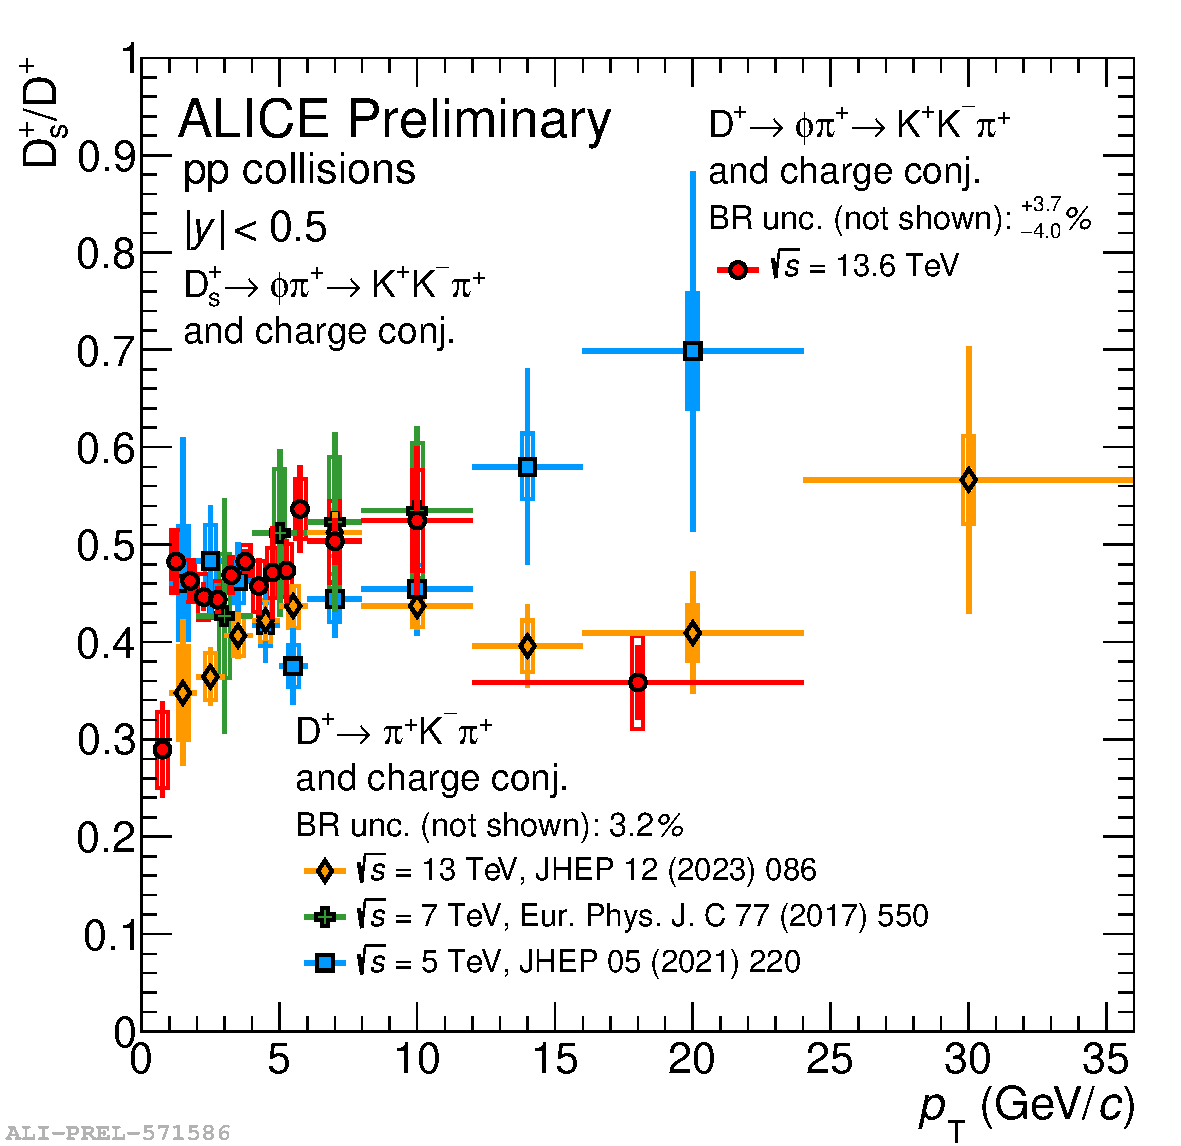
\includegraphics[width=0.7\textwidth]{Figures/Chapter 7/dsoverdpluscomparisonalice_0.pdf}
    \caption{\pt-differential \ds/\dpl production-yield ratio measured at midrapidity ($\lvert y\rvert<0.5$) in pp collisions by the ALICE Collaboration. The results obtained in this Thesis at \thirteen (red) are compared with previous measurements in pp collisions at $\sqrt{s} = 5$, 7, and 13~\tev (blue, green, and orange, respectively).}
    \label{fig:dsdplvsenergy}
\end{figure}

The dependence on the centre-of-mass energy of the \ds/\dpl production-yield ratio can be studied by comparing the results obtained in this Thesis in pp collisions at \thirteen with those obtained, in the same rapidity window of \mbox{$\lvert y\rvert<0.5$}, by the ALICE Collaboration in pp collisions at the centre-of-mass energies of $\sqrt{s} = 5$, 7, and 13~\tev (taken from Refs.~\cite{ALICE:2021mgk,ALICE:2017olh,ALICE:2023sgl}, respectively). The results are shown in Fig.~\ref{fig:dsdplvsenergy}, with red markers being used for the measurement performed in this Thesis. Thanks to the upgrade to the ALICE experimental apparatus~\cite{ALICE:2023udb}, a very large number of minimum-bias events was recorded. In one year of Run~3 data-taking, an integrated luminosity larger than that of the entire Run~2 was collected. In addition, previous measurements of the \ds/\dpl production-yield ratio reconstructed the \dpl meson through the $\dpl\rightarrow\pi^+\mathrm{K}^-\pi^+$ decay channel, which differs from that exploited in this analysis. Despite being characterised by a larger BR of \mbox{$(9.38\pm0.16)\times10^{-2}$}~\cite{pdg}, which leads to a larger amount of reconstructed \dpl mesons, the reconstruction through the same decay channel used for the \ds meson, $\dpl \rightarrow \mathrm{\phi\pi^+ \rightarrow K^+K^-\pi^+}$, allows for the cancellation of some of the systematic uncertainties in the \ds/\dpl ratio. Thereby, a high-precision measurement of the \ds/\dpl production-yield ratio was achieved in this Thesis. Both statistical and systematic uncertainties have been significantly reduced with respect to previous results. Moreover, the \pt reach of the measurement has been extended to lower values, down to $\pt=0.5$~\gevc, and narrower \pt intervals have been analysed. The results from this Thesis present a steeply-increasing \ds/\dpl production-yield ratio between the first two \pt intervals, followed by hints of a decreasing trend with \pt from 1 to 2.5~\gevc and an increasing one for $\pt>2.5$~\gevc. The comparison with previous measurements at midrapidity performed by the ALICE Collaboration at the centre-of-mass energies of $\sqrt{s} = 5$, 7, and 13~\tev show no significant dependence on the centre-of-mass energy, with results being compatible within uncertainties across the whole analysed \pt and \sqs ranges. The comparison with the results obtained at \mbox{$\sqs=13$~\tev} shows that a slightly larger \ds/\dpl production-yield ratio is measured at low \pt at \mbox{\thirteen}. However, the large uncertainties in the previous measurement prevent any firm conclusion on any energy dependence of the observable.


\begin{figure}[tb]
    \centering
    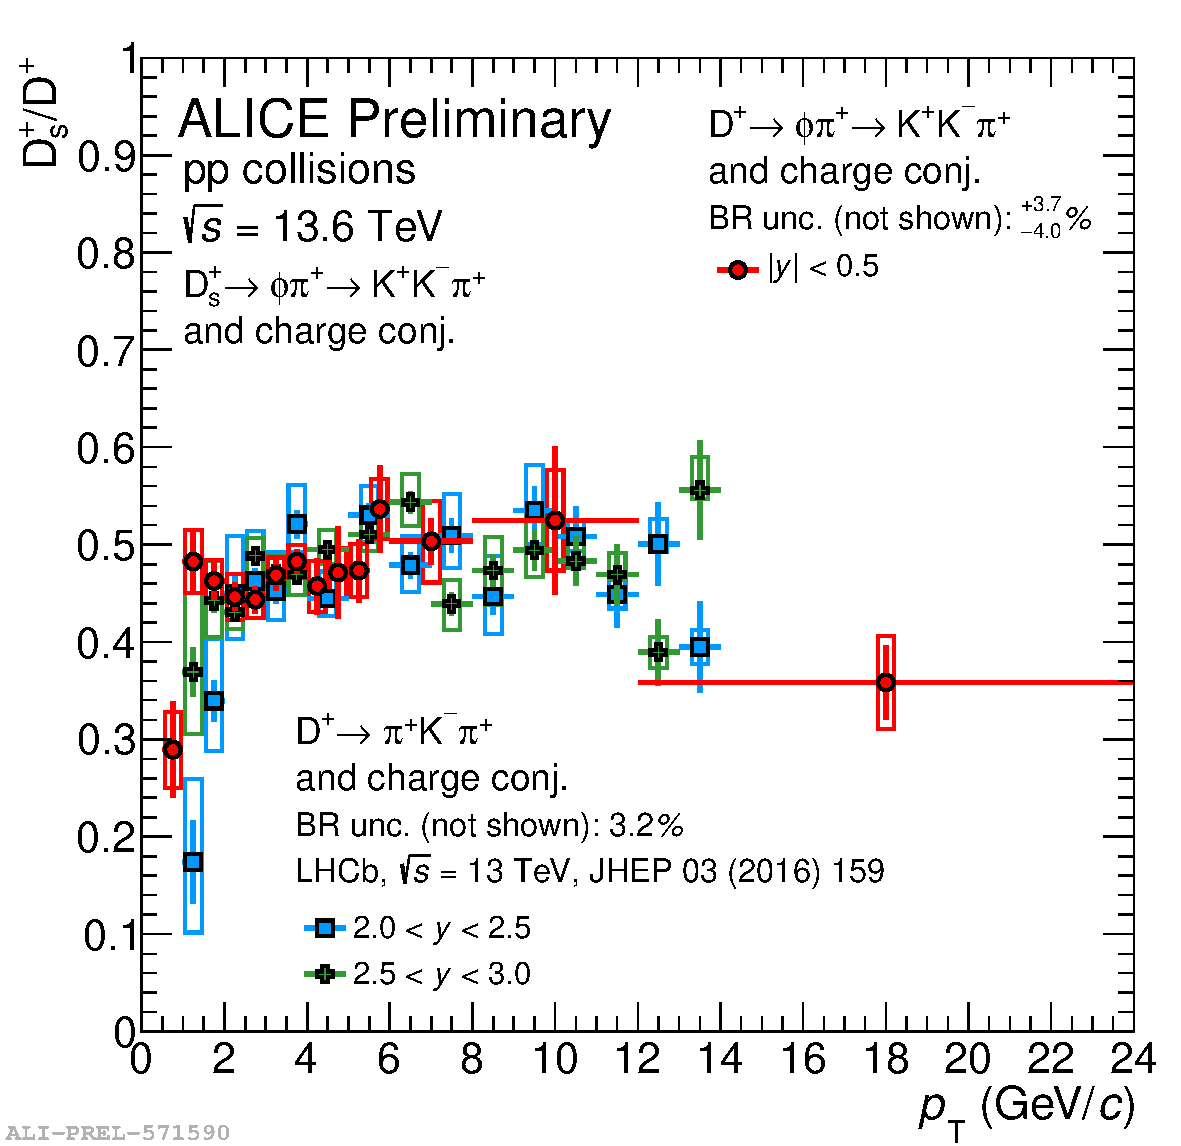
\includegraphics[width=0.7\textwidth]{Figures/Chapter 7/dsoverdpluscomparisonlhcb.pdf}
    \caption{\pt-differential \ds/\dpl production-yield ratio measured at midrapidity ($\lvert y\rvert<0.5$) in pp collisions at \thirteen by the ALICE Collaboration (red), obtained in this Thesis, compared with previous measurement in pp collisions at 13~\tev performed by the LHCb Collaboration in the forward-rapidity intervals of $2.0<y<2.5$ (blue) and $2.5<y<3.0$ (green).}
    \label{fig:dsdplvsrapidity}
\end{figure}
\section{Dependence on rapidity}
The rapidity dependence of the \ds/\dpl produciton-yield ratio can be investigated by comparing the measurement at midrapidity ($\lvert y\rvert<0.5$) performed in this Thesis in pp collisions at \thirteen with those performed at forward rapidities by the LHCb Collaboration~\cite{LHCb:2015swx} at a similar centre-of-mass energy of $\sqs=13$~\tev. Given the energy-independence of the observable which has been discussed above, it is possible to direclty compare the two measurements. Figure~\ref{fig:dsdplvsrapidity} shows the comparison between the \ds/\dpl production-yield ratio measured in this work compared to that from the LHCb Collaboration measured in pp collision in the $2.0<y<2.5$ and $2.5<y<3.0$ rapidity intervals. Thanks to the large dataset available and the reconstruction of the two D-meson species through the same decay channel, the uncertainties of the measurement are significantly smaller than those of the LHCb results across a wide \pt range. In addition, the \pt reach of the measurement is extended to lower values. The results obtained at midrapidity and forward rapidity show a similar trend, with the three \ds/\dpl production-yield ratios compatible within uncertainties across the whole \pt range. The comparison between the results obtained at midrapidity and forward rapidity shows no significant dependence of the \ds/\dpl production-yield ratio on the rapidity of the measurement.
\textcolor{red}{qual è la fisica che possiamo studiare a rapidità a forward? è interessante aspettarsi una dipendenza dalla rapidità?}. 


\section{Comparison to models}
The \ds/\dpl production-yield ratio can be used to test the validity of models describing the production of the two D-meson species, and set constraints on their description of the hadronisation process. Figure~\ref{fig:dsdplvsmodels} presents a comparison between the \ds/\dpl production-yield ratio measured in this Thesis at midrapidity ($\lvert y\rvert<0.5$) in pp collisions at \thirteen with the ALICE experiment (red) and theoretical predictions. 

Predictions from \textsc{Pythia}~8~\cite{Bierlich:2022pfr} are reported using the Monash 2013 tune~\cite{Skands:2014pea} (blue filled boxes), which is tuned on \ee collisions, and colour-reconnections beyond the leading-colour approximation~\cite{Christiansen:2015yqa}. The associated uncertainties are due to the limited amount of simulated pp collision events. Three colour reconnection modes (Mode 0,2,3) are reported in green, violet, and orange, and present similar trends with \pt, with values compatible within uncertainties. \textsc{Pythia}~8 predictions with Monash 2013 tune present a similar dependence on \pt, with a predicted \ds/\dpl production-yield ratio that is larger than that with colour-reconnections beyond the leading-colour approximation. Nonetheless, the four predictions underestimate the measured \ds/\dpl ratio, by a factor of about 1.5 at intermediate \pt. This discrepancy is also observed in the measurement of the \pt integrated $\ds/\mathrm{D^0}$ and $\dpl/\mathrm{D^0}$ production-yield ratio in pp collisions at 5.02~\tev performed by the ALICE Collaboration~\cite{ALICE:2021dhb}, where the same \textsc{Pythia}~8 predictions slightly underestimate the \ds-meson production and overestimate that of \dpl mesons.

Predictions from the Catania~\cite{Minissale:2020bif} model, which describes the production of small droplets of QGP in pp collisions, implementing both the coalescence and fragmentation mechanisms for charm quarks, are reported with a violet dashed line. The model provides a good description of the \ds/\dpl production-yield ratio, managing to reproduce both the magnitude and the increasing trend with transverse momentum at low \pt. 

Lastly, predictions from POWLANG~\cite{Beraudo:2023nlq}, are also reported. Similarly to the Catania model, POWLANG predicts the formation of a small deconfined system in pp collisions, and the same in-medium hadronization mechanism developed for heavy-ion collisions is employed. Two sets of predictions are reported, employing transport coefficients calculated by weak-coupling~\cite{Braaten:1989mz} (Hard-Thermal-Loop, HTL) and lattice-QCD calculations~\cite{Altenkort:2023oms}, using blue and green dashed lines, respectively. Both predictions overestimate the measured \ds/\dpl production-yield ratio, by a factor of about 1.5 at intermediate \pt. In addition, a strong decreasing trend with \pt is predicted, but not observed in the data. These discrepancies are also observed in the measurements of the \pt-differential $\ds/\mathrm{D^0}$ and $\dpl/\mathrm{D^0}$ production-yield ratios in pp collisions at 5.02~\tev performed by the ALICE Collaboration~\cite{Beraudo:2023nlq}, where the POWLANG predictions overestimate the \ds-meson production, with similar differences in the description of the \pt-dependence, while an accurate description of the \dpl meson is achieved.




\begin{figure}
    \centering
    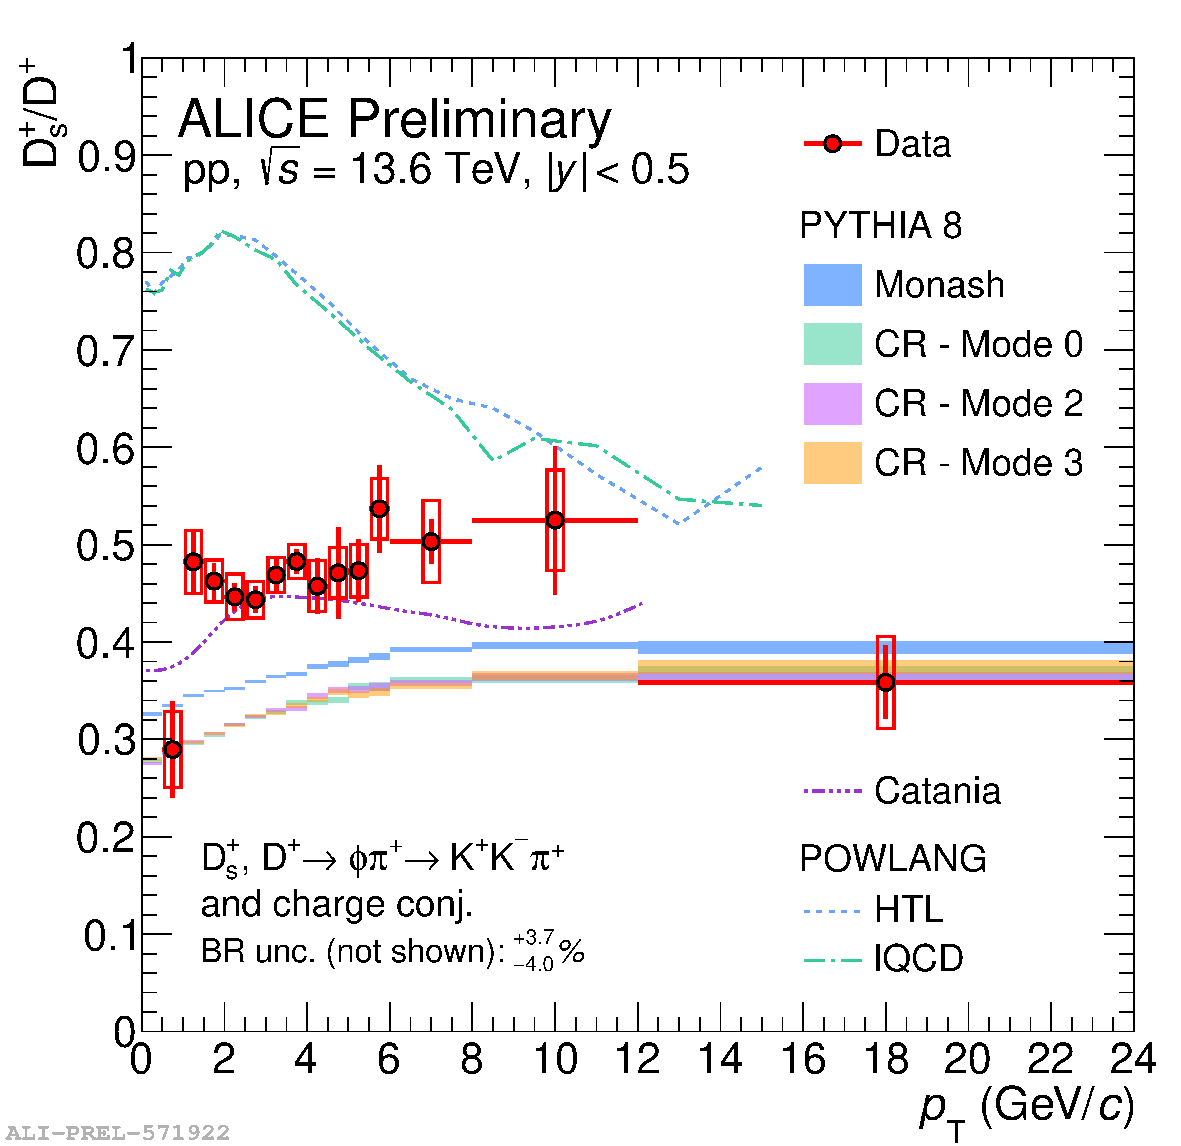
\includegraphics[width=0.7\textwidth]{Figures/Chapter 7/dsoverdpluscomparisonmodels_0.pdf}
    \caption{\pt-differential \ds/\dpl production-yield ratio measured at midrapidity ($\lvert y\rvert<0.5$) in pp collisions at \thirteen by the ALICE Collaboration. The results obtained in this Thesis (red) are compared with the predictions of the FONLL (blue) and GM-VFNS (green) models.}
    \label{fig:dsdplvsmodels}
\end{figure}



%\begin{table}
%    \centering
%    \begin{tabular}{c|cccccc}
%        \toprule
%        Mesone & Massa (\mevcc) & $c\tau (\SI{}{\micro\meter})$ & Canale di %decadimento & BR \\
%        \midrule
%        $\mathrm{D}^0$ & $1864.84 \pm 0.05$ & $123 \pm 3$ & $\mathrm{K}^-\pi^+$ & $%(3.947 \pm 0.030)\%$ \\ 
%        $\mathrm{D}^+$ & $1869.66 \pm 0.05$ & $310 \pm 2$ & $\pi^+\mathrm{K}^-\pi^%+$ & $(9.38 \pm 0.16)\%$ \\
%        & & & $\phi\pi^+\rightarrow \mathrm{K}^+\mathrm{K}^-\pi^+$ & $(2.69^{+0.07}_%{-0.08})\times10^{-3}$ \\
%        $\mathrm{D^+_s}$ & $1968.35 \pm 0.07$ & $150 \pm 6$ & $\phi\pi^+\rightarrow %\mathrm{K}^+\mathrm{K}^-\pi^+$ & $(2.21 \pm 0.06)\%$ \\
%        \midrule
%        $\mathrm{B^0}$ & $5279.72 \pm 0.08$ & $455 \pm 12$ & $\mathrm{D}^-\pi^+$ & $%(2.51 \pm 0.08)\times10^{-3}$ \\
%        & & & $\mathrm{D}^-\mathrm{K}^+$ & $(2.05 \pm 0.08)\times10^{-4}$ \\
%        $\mathrm{B^+}$ & $5279.41 \pm 0.07$ & $491 \pm 12$ & $\mathrm{\overline{D}}%^0\pi^+$ & $(4.61 \pm 0.10)\times10^{-3}$ \\
%        & & & $\mathrm{\overline{D}}^0\mathrm{K}^+$ & $(3.64 \pm 0.15)\times10^{-4}$ %\\
%        $\mathrm{B^0_s}$ & $5366.93 \pm 0.10$ & $456 \pm 15$ & $\mathrm{D_s^-}\pi^%+$ & $(2.98 \pm 0.14)\times10^{-3}$ \\
%        & & & $\mathrm{D_s^\mp}\mathrm{K}^\pm$ & $(2.25 \pm 0.12)\times10^{-4}$ \\
%        \bottomrule
%    \end{tabular}
%\end{table}